\chapter{Experimental Evaluation}
\label{chapter:evaluation}


\section{Environment setup}
��\begin{table}[h]

    \centering

    % [] o�:y?���� list of tables ??????��?

    % {} o�:y?����h�<h
N�e??????��?

    \caption[Experimental setup]{Experimental setup}

    \label{table:setup}

    \begin{tabular}{p{45mm}p{50mm}}

    \toprule[1.1pt]

    \multirow{1}{*}{Number of organizations} & 5\\

    \midrule

    \multirow{1}{*}{Number of nodes} & 2\\

    \midrule

    \multirow{1}{*}{Number of sealers} & 1\\    

    \midrule    

    \multirow{1}{*}{State database} & LevelDB, key-value storage\\

    \midrule

    \multirow{1}{*}{Consensus mechanism} & Proof of authority (PoA)\\

    \midrule

    \multirow{1}{*}{Block time} & 1s\\

    \midrule

    \multirow{1}{*}{Difficulty} & 0x1\\

    \bottomrule[1.1pt]

    \end{tabular}

    \end{table}
We set up an experimental environment on a PC running Ubuntu 18.04 and Intel i7-9700 CPU @ 3.00GHz. We deploy the blockchain network in Docker host with Geth tools. Table~\ref{table:setup} summarizes Ethereum blockchain parameters in our experiment. The \(TSP\)'s server and \(Org\)'s server run within a Docker container for local testing. For example, a bank system we used for evaluation includes the following servers: LDAP server, web server. And each web server will interact with a remote Ethereum node through web3js. Although the TSP's system maintains an LDAP server, it is only for record user's information and doesn't responsible for registration. It only allows blockchain-based login without providing username and password. \par
In our proposed ecosystem, we use consortium blockchain as our blockchain network. The consortium blockchain is a "semi-private" system and works across different organizations. This blockchain is only used internally for a certain organization or TSP. It needs to pre-allocate several nodes as sealers that are responsible for mining blocks. Other nodes can send transactions, call smart contract, but they don't have right to mine blocks. In tern of consensus algorithm, Proof of Work (PoW) consensus algorithm is the most reliable and secure, it can provide a trustless economic system. Although it secure and trustless, PoW has the worst performance and has lower tps. In our experiment, we adopt Proof of Authority (PoA) that relies on a limited number of sealers, and it is regarded as an effective and reasonable solution for our scenario.
\section{Gas consumption}
\begin{table}[h]
    \centering
    % [] 顯示在 list of tables 的文字
    % {} 顯示在表格上方的文字
    \caption[Gas consumption]{Gas consumption}
    \label{table:gasUsed}
    \begin{tabular}{p{45mm}p{30mm}}
    \toprule[1.1pt]
    Function/Contract   & Gas used\\
    \midrule[1.1pt]
    \multirow{1}{*}{AddUser-create} & 97574\\
    \midrule
    \multirow{1}{*}{AddUser-append} & 36435\\
    \midrule
    \multirow{1}{*}{Bind} & 1390534\\
    \midrule
    \multirow{1}{*}{Authorize} & 49263\\
    \midrule
    \multirow{1}{*}{Revoke} & 19284\\
    \midrule
    \multirow{1}{*}{Authorize-all} & 46580\\    
    \midrule
    \multirow{1}{*}{Revoke-all} & 16625\\
    \midrule
    \multirow{1}{*}{New $Omgr$} & 4494629\\
    \midrule
    \multirow{1}{*}{New $ACMgr$} & 1660077\\    
    \bottomrule[1.1pt]
    \end{tabular}
    \end{table}
The Ethereum gas refers to the computational expense on the Ethereum network. The amount of gas consumption is determined by the difficulty of calculation. Table~\ref{table:gasUsed} shows the gas consumption of each smart contract function and contract deployment fee. There is a significant difference between the two type function calls. In the case of the deployment contract, it will spend more gas such \textit{bindAccount}. In other words, if the function does not involve complex logic or deployment, it will consume less gas such as \textit{addUser}, \textit{authorize}, \textit{revoke}.

\section{Throughput}
\begin{figure}[htb]
    \centering
    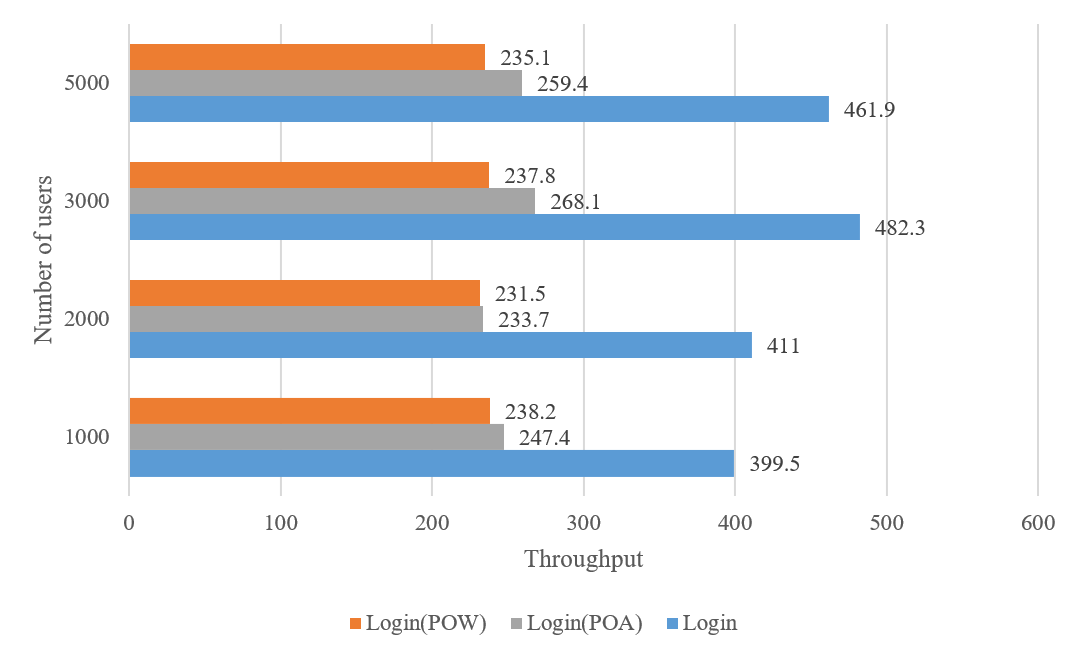
\includegraphics[height=!,width=0.9\linewidth,keepaspectratio=true]{figures/login-throughput.png}
    \caption{{\footnotesize Number of users vs throughput}}
    \label{fig:loginThroughput}
\end{figure}

\begin{figure}[htb]
    \centering
    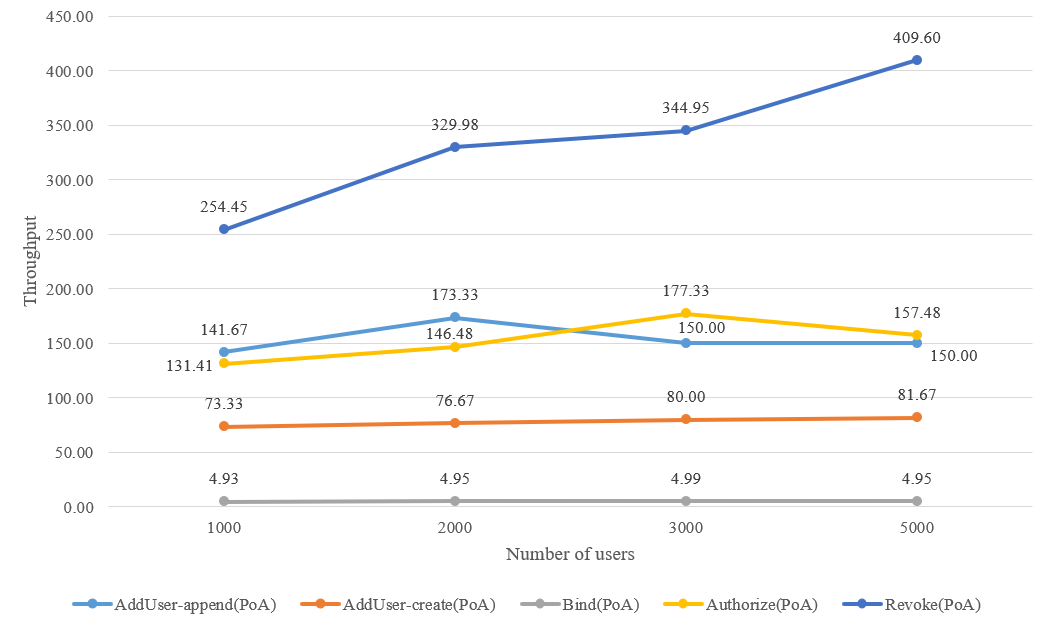
\includegraphics[height=!,width=1\linewidth,keepaspectratio=true]{figures/smart_contract_tps.png}
    \caption{{\footnotesize Each function of smart contract}}
    \label{fig:contract_tps}
\end{figure}

\begin{figure}[htb]
    \centering
    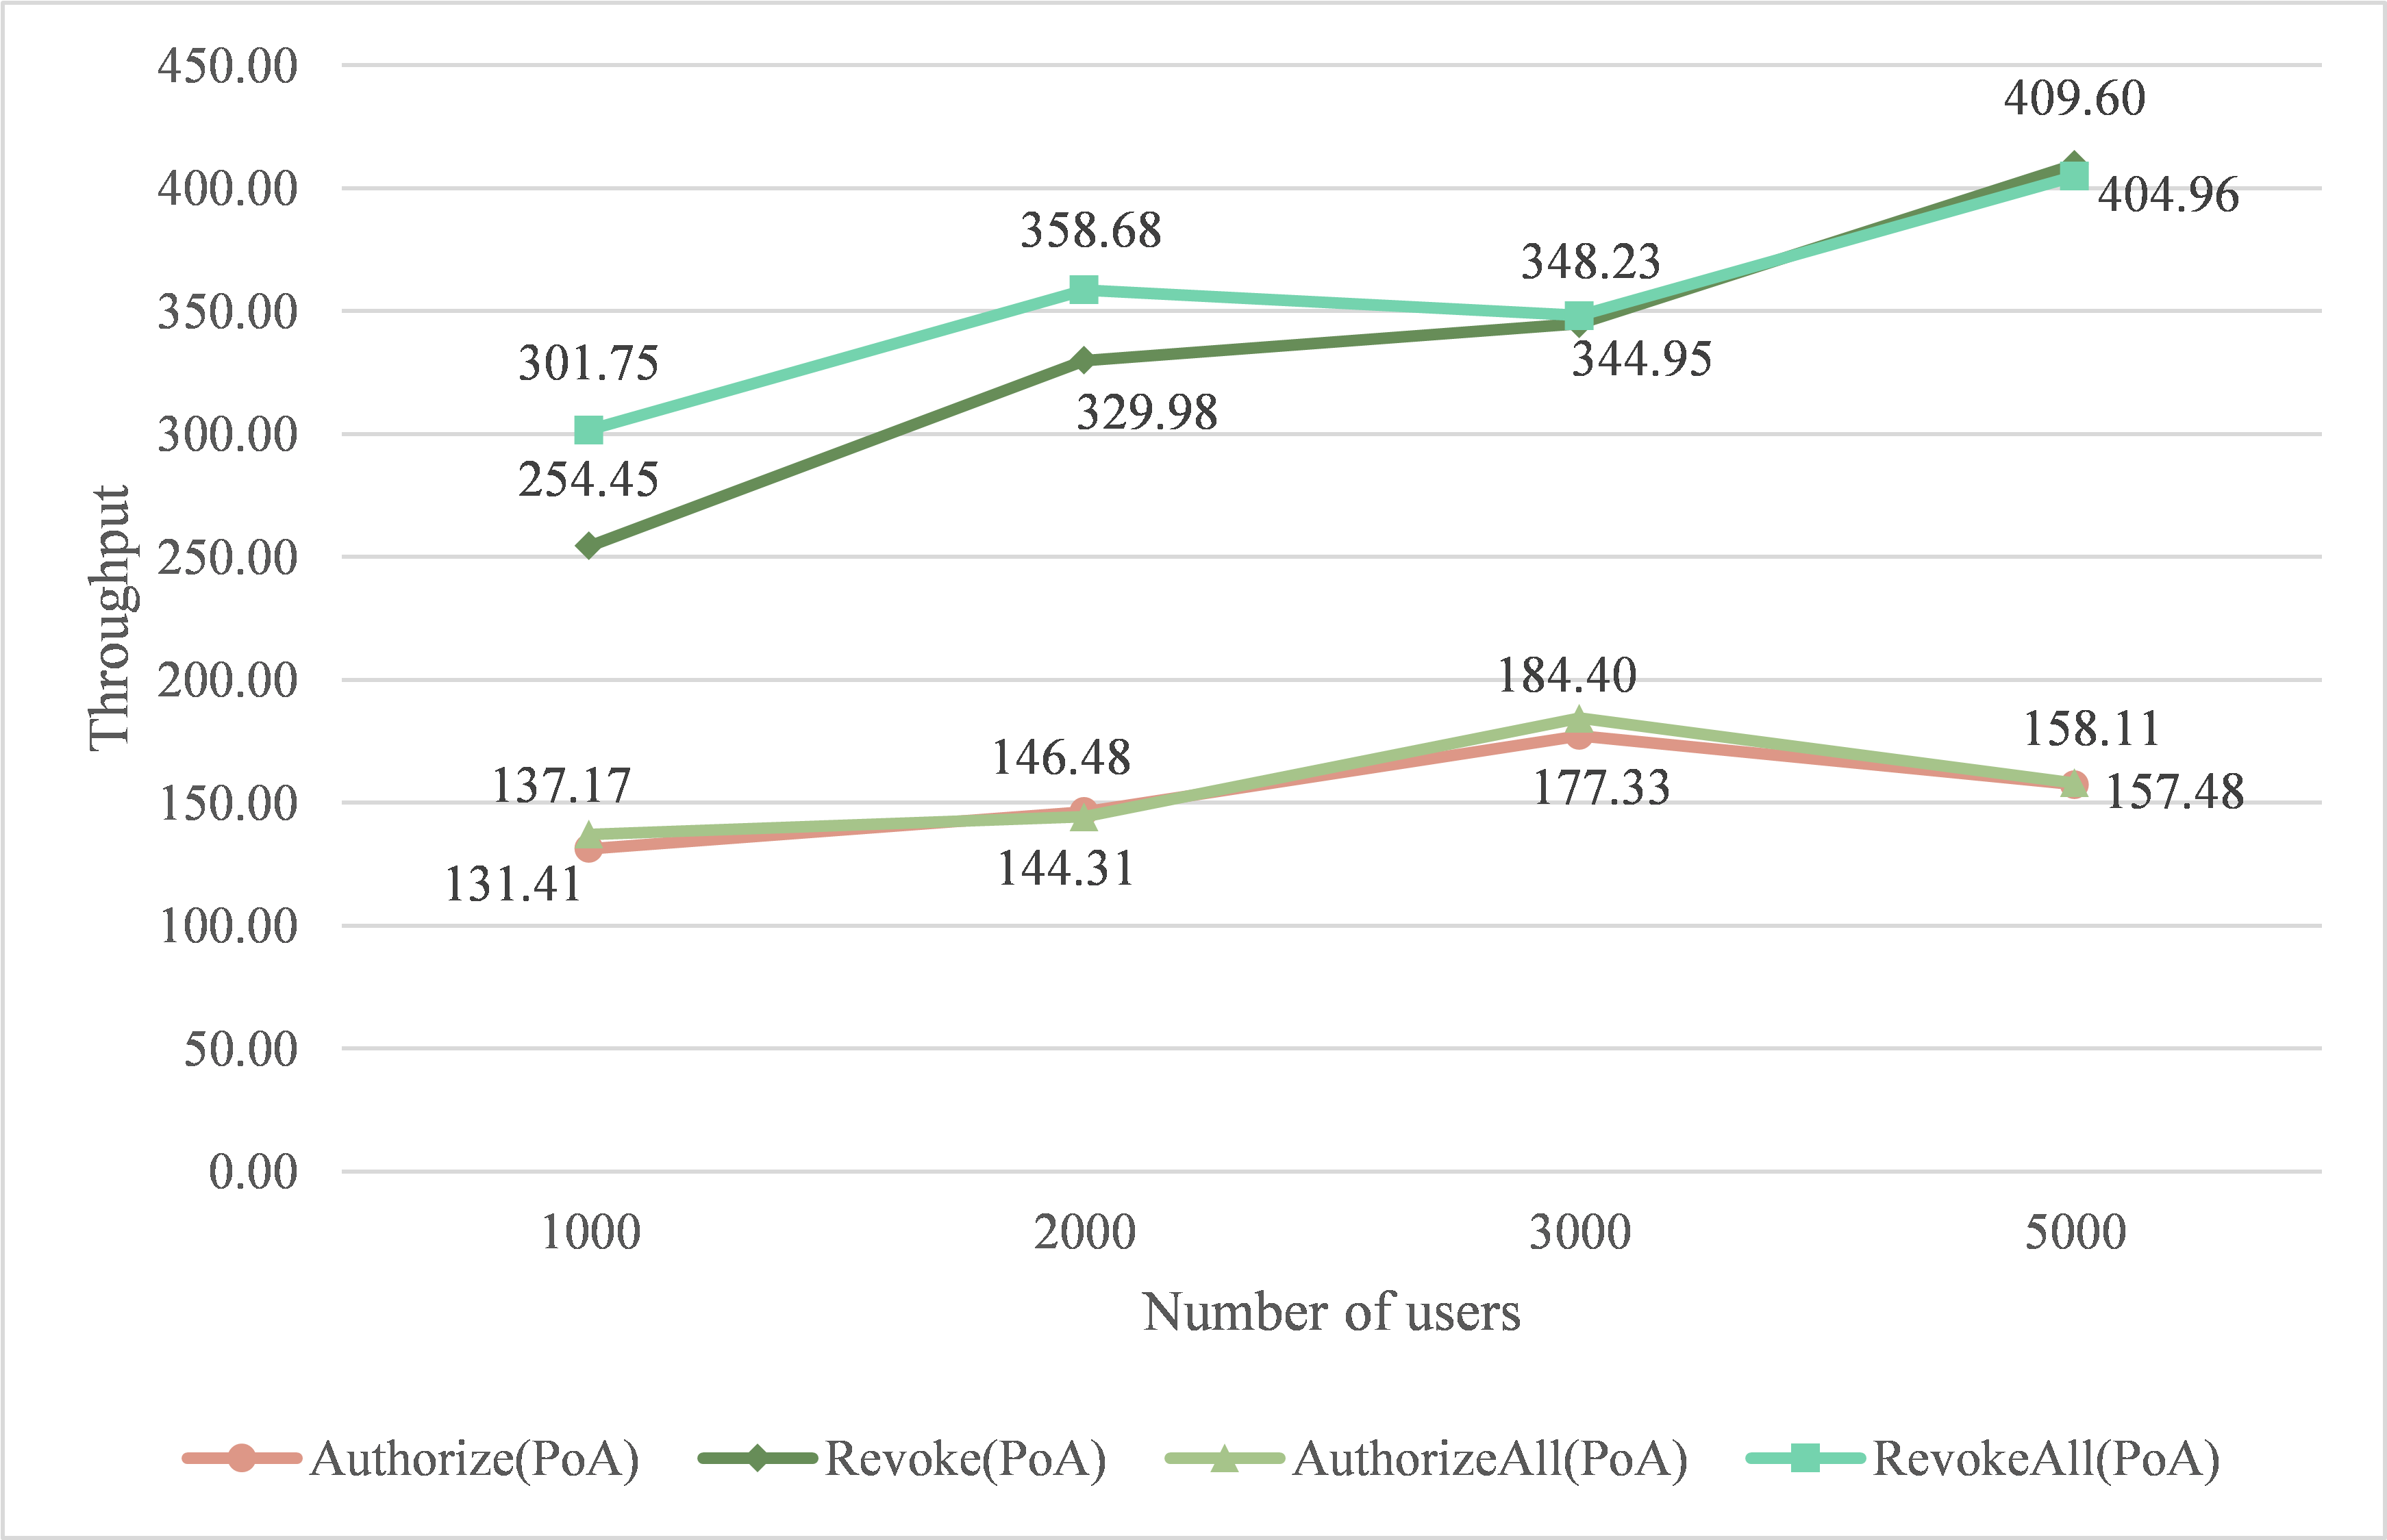
\includegraphics[height=!,width=1\linewidth,keepaspectratio=true]{figures/authorize_comparsion.png}
    \caption{{\footnotesize Comparsion of two modes}}
    \label{fig:authorize_compare}
\end{figure}

\begin{figure}[htb]
    \centering
    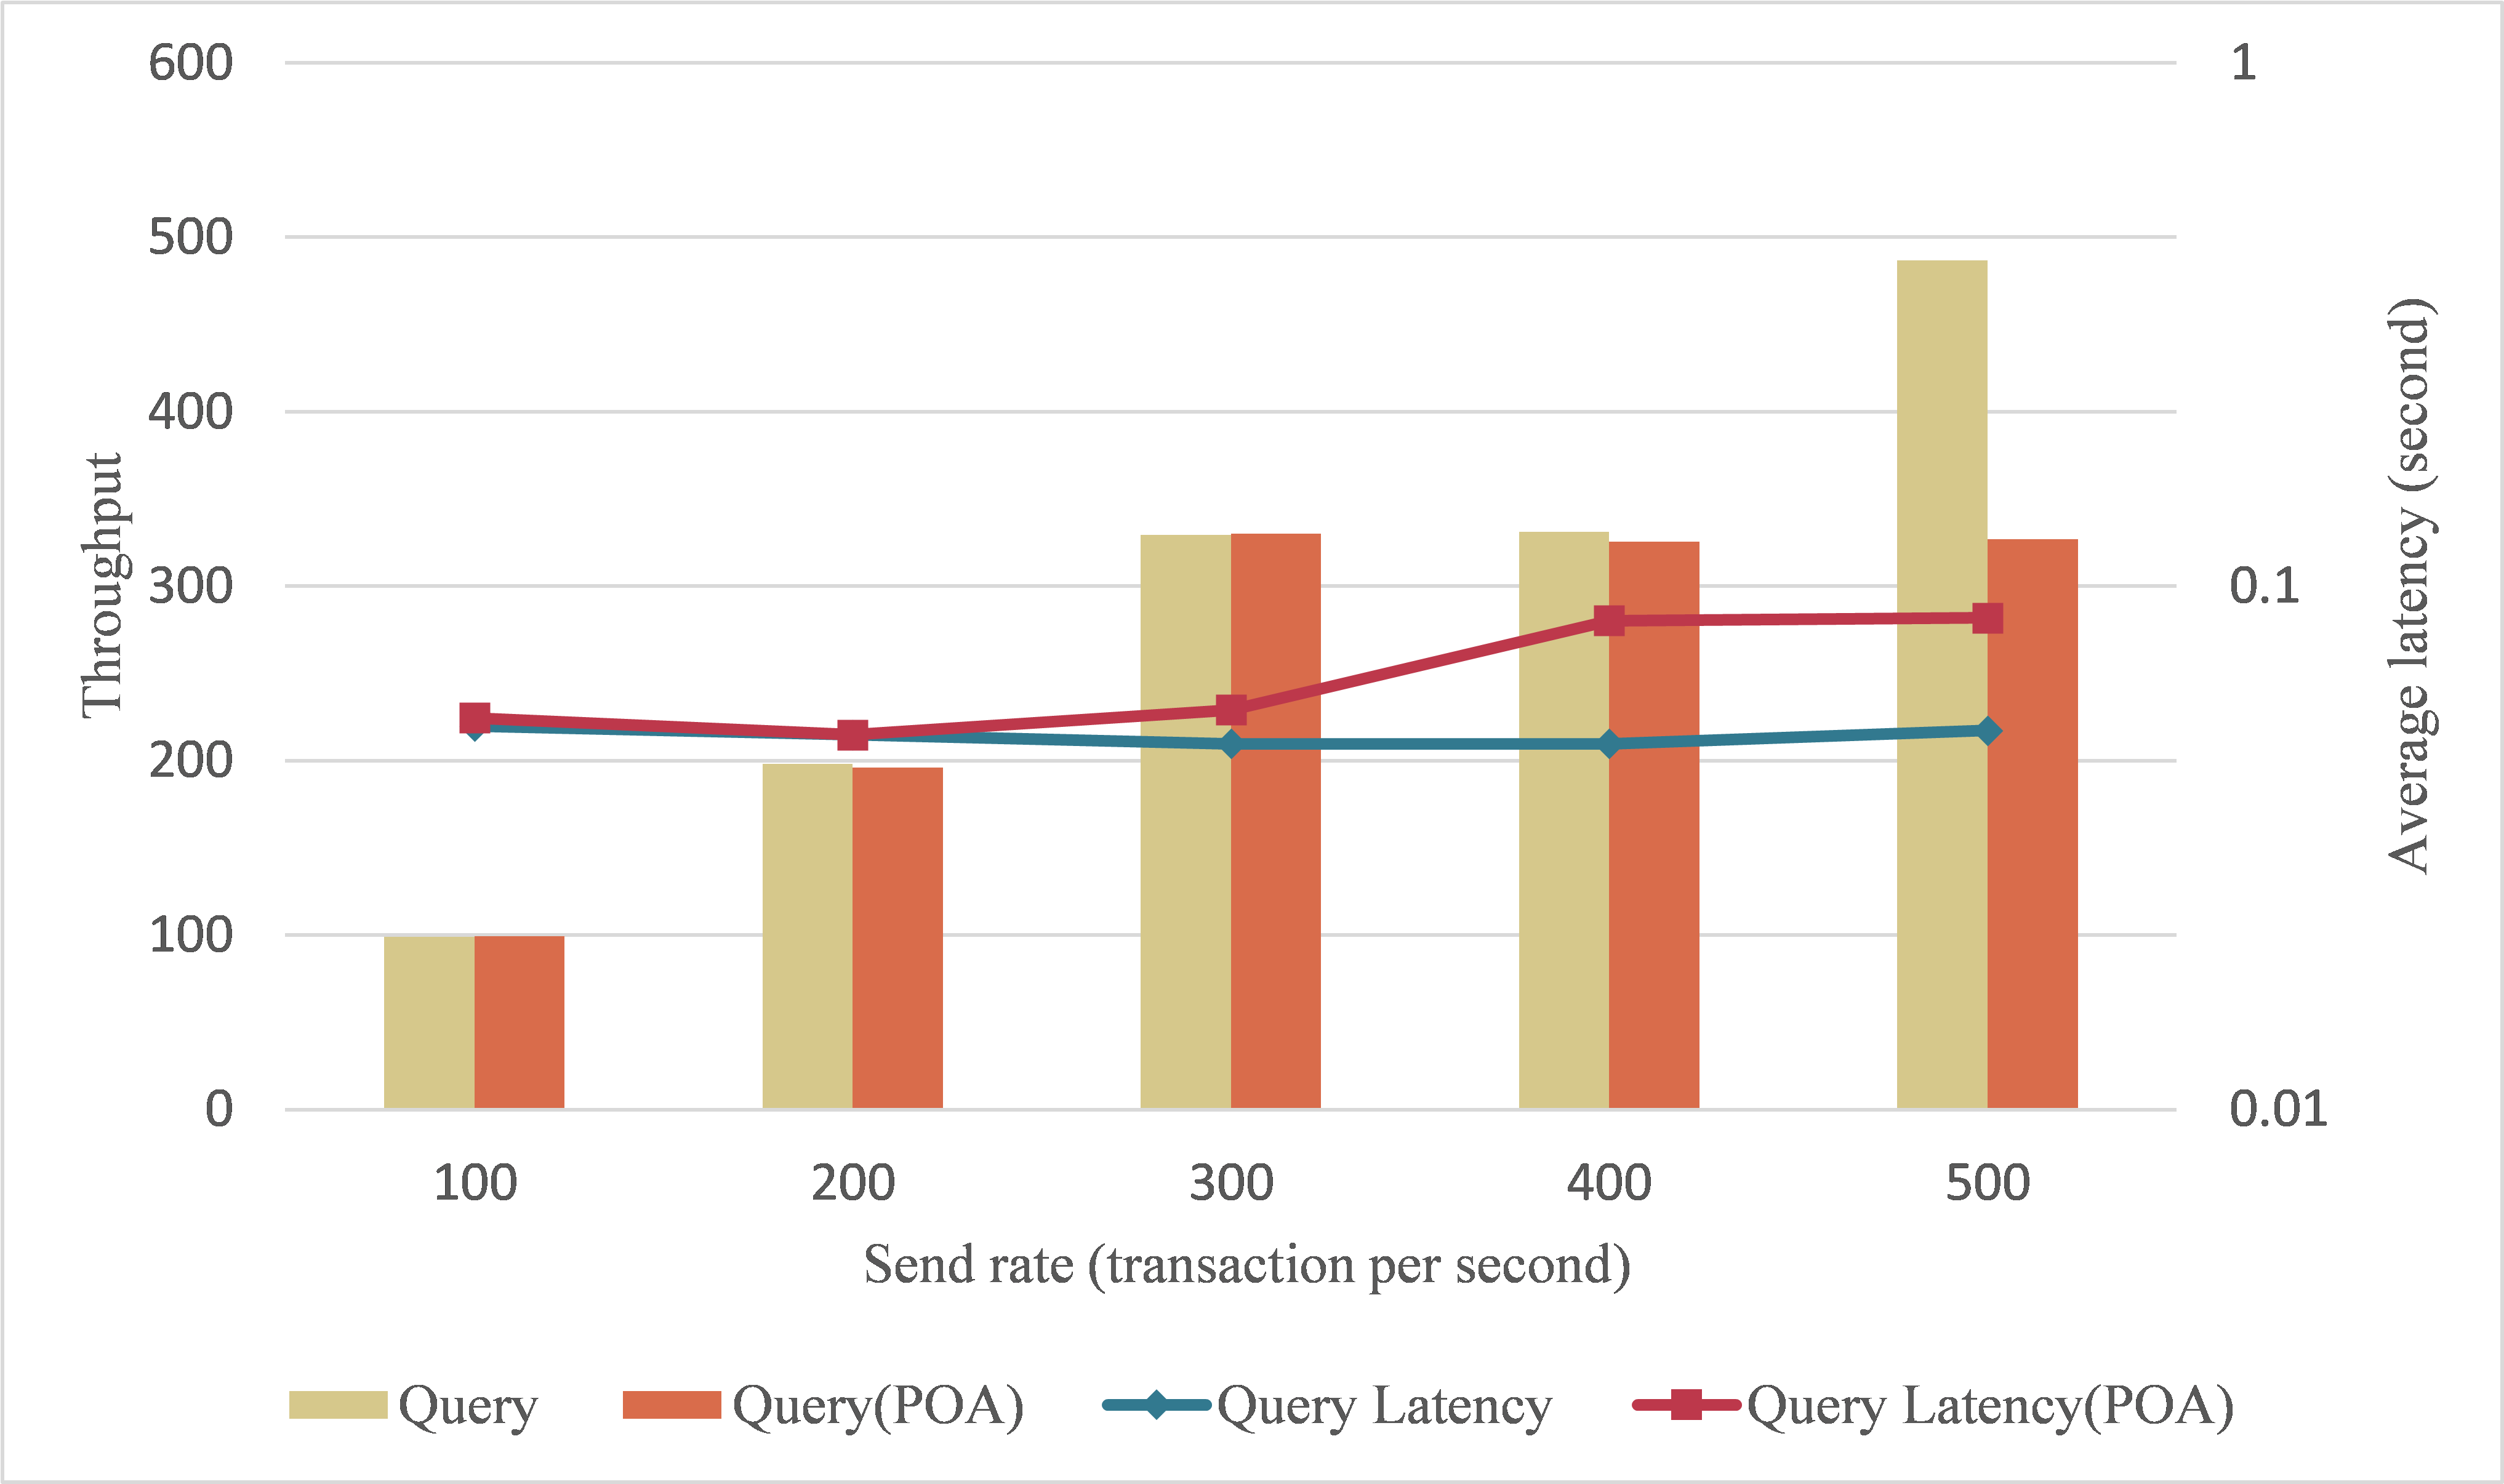
\includegraphics[height=!,width=1\linewidth,keepaspectratio=true]{figures/query.png}
    \caption{{\footnotesize Query with JWT and blockchain}}
    \label{fig:query}
\end{figure}